\documentclass{report}
\usepackage{epsfig,graphics,fancybox,amsmath,hyperref,ulem,tabularx,color,graphicx,multirow,colortbl,soul,undertilde,wrapfig,multicol}
\newcommand{\hili}[1]{\colorbox{yellow}{#1}}
\newcommand{\Yb}{\mathbf{Y}}
\newcommand{\Xb}{\mathbf{X}}
\newcommand{\ind}{\mbox{\large $I$}}
\newcommand{\sumi}{\sum_{i=1}^n}
\newcommand{\betaB}{\mbox{\boldmath$\beta$}}
\newcommand{\alphaB}{\mbox{\boldmath$\alpha$}}
\newcommand{\Rhotau}{\mbox{\large$\rho$}_{\tau}}
\newcommand{\CinP}{\stackrel{P}{\longrightarrow}}
\newcommand{\To}{\longrightarrow}	
\newcommand{\bi}{\begin{itemize}}
\newcommand{\ei}{\end{itemize}}
\newcommand{\head}{\textbf{\blue{}}}
\newcommand{\be}{\begin{enumerate}}
\newcommand{\ee}{\end{enumerate}}


\normalem
%\input /home/jaosborn/research/mymacs.tex
\def\defn{\noindent\underline{Definition}: }
\def\gmeanb{\bar{y}_{+++}}
\def\tmean#1{\bar{y}_{#1+}}
\def\Tmean#1{\bar{Y}_{#1+}} 
\def\h0sim{\stackrel{H_0}{\sim}}
\def\abg#1{(\alpha\beta\gamma)_{#1}}

\makeatletter
\def\hlinewd#1{%
\noalign{\ifnum0=`}\fi\hrule \@height #1 %
\futurelet\reserved@a\@xhline} 
\makeatother

\setlength{\textwidth}{6.5in}
\setlength{\textheight}{8.5in}
\setlength{\parindent}{0pt}

\begin{document}
\setlength{\topmargin}{0pt}
\setlength{\oddsidemargin}{0pt}
%\tableofcontents

\newpage
\pagenumbering{arabic}
\Huge ST 512 - Design of Experiments Supplement\large
\begin{center}\large\textbf{Readings: Chapter 2 (for 2.2/2.3 read if interested)}\\
\normalsize \end{center}
\large ~\hrulefill
~\\
\normalsize This class is about analyzing data.  As scientists, most of the time this data will come from a designed experiment, but the methods used for analysis are also useful for observational studies.  However, the conclusions drawn will differ!  Let`s define what me mean by experimental and observational study.\\~\\

\textcolor{red}{Observational Study}
%\underbar{~~~~~~~~~~~~~~~~~~~~~~~~~~~~~~~~~~~~} 
researchers does not interfere or intervene in the process of collecting data. 
\begin{itemize}
\item Ex: measuring political beliefs in using a poll, measuring yield of a crop based on rainfall
\end{itemize}
\textcolor{red}{Experimental Study}
%\underbar{~~~~~~~~~~~~~~~~~~~~~~~~~~~~~~~~~~~~} 
researchers manipulate the conditions in which the experiment is done. 
\begin{itemize}
\item Ex: assigning different fertilizers and irrigation method and measuring crop yield, assigning temperatures of water to tanks containing a fish and observing weight gain
\end{itemize}
~\\
Big difference in conclusions drawn!
\begin{itemize}
\item Cannot usually infer causation from observational experiments, but you can from a well-designed experiment.
\item Experiments are not always feasible or ethical.  i.e. cannot assign people to smoke a pack a day or have expectant mothers drink a certain amount of alcohol.
\end{itemize}
~\\~\\
To describe the methods for creating a well-designed experiment, we first need some definitions.
\begin{itemize}
\item \textbf{Response Variable} - Variable of interest that characterizes performance or behavior.
\item \textbf{Explanatory Variables} - Variables that determine the study conditions (can be quantitative or categorical).
\item \textbf{Factor} - Explanatory variable of interest.
\item \textbf{Level} -	The specified value of a factor (or explanatory variable).
\item \textbf{Confounding Variable} - Explanatory variable (not of interest) that may mask (or enhance) the effect of a factor.
\item \textbf{Covariate} - Quantitative confounding variable.
\item \textbf{Treatment} - A specific experimental condition, either the level of a factor (if only 1 factor) or the combinations of levels from a number of factors.
\item \textbf{Experimental units (EUs)} - Units on which the treatments are assigned.
\item \textbf{Measurement (Observational) units} - Units on which values are observed (often the same as EUs, but not always).
\item \textbf{Replicate} - Name given to EUs that receive the same treatment.
\item \textbf{Control Treatment} - Benchmark treatment sometimes necessary for comparison (to avoid the \textit{placebo effect}).
\item \textbf{Experimental Error} - Used to describe the variation in response among EUs that are assigned the same treatment.
\end{itemize}

\textbf{Example: } An experiment was run to determine the effects of adding phosphorous ($0, 147, 294, 441$ $kg/m^2$) and nitrogen ($0, 45, 90, 135$ $kg/m^2$) to the soil of a certain type of grass (a Miscanthus species).  The growth of the plant was of interest and at the end of the growing period the plant was dried and the weight recorded with the final measurement being recorded in megagram per hectare ($0.1$ $kg/m^2$).  Four plots of grass were used in total.  Within each plot, each combination of phosphorous and nitrogen was observed.  The plots were arranged in a large field in a 4x1 rectangle (north to south).  There is a possibility of a water gradient as a stream runs to the north of the field.   A partial data table is given here: 
\begin{center}
\begin{tabular}{c|c|c|c}
\hline
Plot	&P	&N&	Dry yield\\
\hline
1&	0&	135&	1.95\\
1&	0&	45&	3.51\\
1&	0&	90&	2.87\\
1&	0&	0&	2.88\\
1&	294	&45&	2.37\\
1&	294	&0&	3.5\\
1&	294	&135&	3.55\\
1&	294&	90&	4.4\\
...&...&...&...\\
\end{tabular}
\end{center}
Let`s identify (if possible) the response, explanatory variable(s), factor(s), level(s), confounding variable(s), treatment(s), number of replicates, experimental units, and observational units.  %\\~\\~\\~\\~\\~\\~\\~\\~\\~\\~\\~\\~\\~\\
\textcolor{red}{\\
Response: Y = Growth of plant\\
Explanatory Variable(s): Phosphorous, Nitrogen, Plot\\
Factor(s): Phosphorous, Nitrogen\\
Level(s): For Phosphorous - (0, 147, 294, 441), For Nitrogen - (0, 45, 90, 135)\\
Confounding Variable(s): Plot\\
Treatment(s): Combos of Phos and Nitrogen Levels - (0,0), (0,45), ..., (441,90),(441,135)\\
\# of replicates: 4\\
EUs: Areas of the plots that were assigned the treatments\\
OUs: Same as EUs here.\\}
(See example 2.4/2.7 and the resulting discussion for more practice)

\newpage

Notice that many of the response values are different.  What is causing them to be different?\\~\\
Sources of Variation in the responses of an experiment:
\begin{enumerate}
\item \textbf{Treatment effect} - we hope there is an effect due to the variables we are setting
\item \textbf{Identified confounding variables} - We record some variables that are not of interest, but we think may have an effect on the response.
\item \textbf{Unidentified sources (these make up the Experimental Error or error variation)} -
		\begin{enumerate}
			\item Inherent variability in experimental units - Experimental units are different! \\
		Ex: No two people, paper towels, concrete blocks, or even lab rats are exactly the same.\\
		Consequence: Experimental units respond differently to the same treatment
			\item Measurement error - Multiple measurements of a same experimental unit typically contain error.\\
			If the same experimental unit is measured more than once, will the value be the same?\\
			Ex: Blood Pressure, Break a water sample in two, measure each for bacteria
			\item Variations in applying/creating treatments\\
		The treatment is not clearly defined, leaving room for interpretation.  \\
			Ex:  Two researchers mix concrete, one stirs for 10 minutes and one for 20 minutes, will they come out exactly the same? Temperature is of interest but two ovens don`t heat exactly the same, etc.
			\item Effects from any other extraneous (or lurking) variables - Extraneous variables are those variables that are not part of the treatment, but may influence the response.\\
			Ex: For the oven example, the experiment is done over the course of several days.  There may be slight differences due to humidity changes.
		\end{enumerate}
\end{enumerate}
Let`s identify these in the grass growth example.
%\\~\\~\\~\\~\\~\\~\\~\\~\\~\\~\\~\\~\\~\\~\\~\\~\\~\\~\\~\\~\\~\\~\\~\\
\textcolor{red}{\\
(a) Each area of grass might differ causing the responses to differ\\
(b) When drying the grass for weighing, maybe you lose some or the scale varies\\
(c) For some plots the Phos is added first then the Nitrogen, for others they Phos and Nitrogen are mixed then added.  This  may cause a difference in response\\
(d) Could be many things such as sun variance across plots or neighboring area differs (trees for other grass), etc.\\}
(See example 2.5/2.6 and the resulting discussion for more practice)

\newpage

No matter how hard we try, some experimental error will remain. What we can do is use good experimental design techniques to ensure our study is valid.\\~\\
DOE is about creating the optimal experiment to determine the effects of different treatments.  Different types of experimental designs are then analyzed differently.\\~\\
\textbf{Pillars of Experimental Design}\\
\begin{enumerate}
		\item 
		%\underbar{~~~~~~~~~~~~~~~~~~~~~~~~~~~~~} 
		\textcolor{red}{Randomization}
		- means that the treatments are randomly allocated to the EUs.
			\begin{enumerate}
				\item Every EU has a chance to get a different treatment, so helps protect the results of the analysis against a systematic influence of lurking variables.  
				\item Allows the observed responses to be regarded as a random sample.
			\end{enumerate}
		Note: Different randomization schemes lead to different statistical analyses.\\~\\
		%\underbar{~~~~~~~~~~~~~~~~~~~~~~~~~~~~~~~~~~~~~~~~~~~~~~~~} 
		\textcolor{red}{Completely Randomized Design}
		- for t treatments, replicated $n_t$ times each, use a random number generator to assign the treatments to the EUs.\\~\\
		Most basic randomization design - assumes all EUs are exchangeable.\\~\\~\\~\\~\\~\\~\\~\\~\\
		\item 
		%\underbar{~~~~~~~~~~~~~~~~~~~~~~~~~~~~~} 
		\textcolor{red}{Replication}
		- Repetition of an experiment using a large group of subjects to reduce chance variation in the results
\begin{enumerate}
				\item Allows us to generalize the results to the population and increases reliability of conclusions. 
				\item Allows an estimate of variability (an estimate of experimental error) not due to the treatment effect.
			\end{enumerate}
Note: Replication does not mean that we measure the same EUs multiple times, this is called repeated measures.  Observations from repeated measures experiments cannot 	usually be considered independent.
%\noindent\textit{Ideally as many EUs as we can afford.  Think if we had 3 diets and 3 EUs.  Diet 1 was better than diet 2 and diet 3, not a very reliable conclusion, perhaps person 1 just loses weight more easily.  Now if 100 people at each diet and on average diet 1 was much better, more reliable conclusion.}\\~\\
%\noindent\textit{By averaging over the many observations we can reduce the effects of measurement error and error in applying/creating the treatments.}\\~\\
\newpage
		\item \textbf{Methods for accounting for/reducing experimental error}
		\begin{enumerate}
			\item Controlling Variables - holding certain variables constant across the EUs\\
			Decreases generalizability, but reduces experimental error.\\~\\
\noindent\textit{We`re not interested in the effects of these variables on the response.  These variables affect the response in exactly the same manner, so that we	don`t see the effects on the conclusions. We don`t get information on what happens at levels other than the fixed one.}
		\item Blocking - Divide subjects with similar characteristics into `blocks', and then within each block, randomly assign subjects to treatment groups.\\~\\
			Blocks - Groups of EUs sharing a common level of a confounding variable.\\
\begin{center}
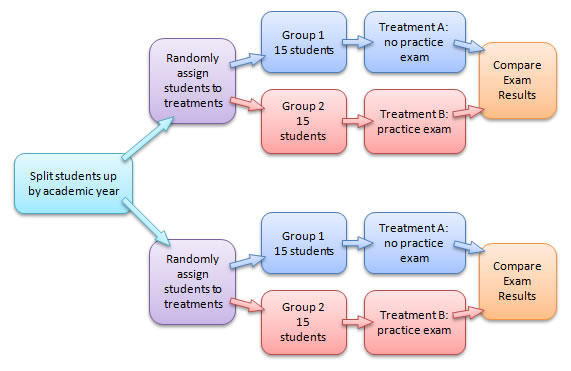
\includegraphics[scale=0.5]{block.jpg}
\end{center}
			Similar to controlling, but allows for increased generalizability.  EUs within a block are very similar (decreases experimental error there as all the EUs in a block are affected similarly by the confounding variable).  By having enough blocks to cover the range of the population you can still generalize.)
		\end{enumerate}
	\end{enumerate}
		\noindent\textit{There are also methods for dealing with some explained experimental error during the analysis stage - Namely ANCOVA.\\~\\
		These ideas are very important.  Unless you are well versed in statistical methods and ideas you should consult a statistician before investing time and money in an experiment.\\
`A poorly designed study can never be saved, but a poorly analyzed one has the possibility of being reanalyzed.'}

\end{document}



\chapter{ST 511 - Review}
\input Review




